%% MPI collectives
%% MPI communicators
%% Barrier (N/2, N/4, ..)
%%.  linear
%%.  tree
%% Broadcast (1, 2, 4..)
%% Reduction
%% MPI_Barrier
%% MPI_Broadcast
%% MPI_Reduce
%% MPI_Allreduce
%% MPI_Gather
%% MPI_Allgather
%% MPI_Scatter
%% MPI_Allscatter
%% MPI_Alltoall

\minitoc

In Lecture \ref{MPIIntro.chap} we introduced the Message Passing Interface and focused on point-to-point communication patterns used in distributed computing. By combining several point-to-point communications we can form a wide variety of communication patterns between multiple MPI processes that occur over and over again when writing parallel code. 

In this lecture we describe some very common communication patterns that involve (potentially) all the MPI processes. In each case we develop an implementation using MPI point-to-point communications and then introduce the equivalent built-in MPI collective communication function.

Example collective communication patterns include:

\begin{table}[htbp!]
    \centering
    \begin{tabular}{c|p{3in}|p{1in}} \hline
    {\bf Operation} & {\bf Description} & {\bf MPI function} \\ \hline
    Broadcast & One process sends a message to all other processes & \texttt{MPI\_Bcast} \\ \hline
    Sum reduction & All processes collaborate to sum up a value held by each process with the final result available to one process & \texttt{MPI\_Reduce} \\ \hline
    Barrier & All processes must enter the barrier function before any process can leave the barrier function & \texttt{MPI\_Barrier} \\
   \hline 
   All to all & All processes send a message (of the same length) to all other processes & \texttt{MPI\_Alltoall} \\ \hline
   \end{tabular}
    \caption{Summary of MPI collective communications.}
    \label{mpiCollectives.tab}
\end{table}

%% home grown broadcast
\section{Broadcast operation}

The first collective communication pattern we consider is the broadcast: one process (which we will call the root process, and for simplicity we will nominate process rank zero as the source process) sends a message to all the other processes. The simplest way to do this:  the root process sequentially sends the message to all other ranks. If there are $P$ processes then it will take the root process $P$ message rounds to complete the broadcast. However, there is a missed opportunity here. After rank one receives the first message from the root process it does not pass the message on, selfishly keeping the incoming message to itself.

We can reduce the number of messages sent by any single process by  borrowing the ``phone tree'' that schools used to use to send out messages to parents. In Figure \ref{broadcast.fig} we illustrate how the tree based broadcast can be organized. 

\begin{figure}[htbp!]
    \centering
    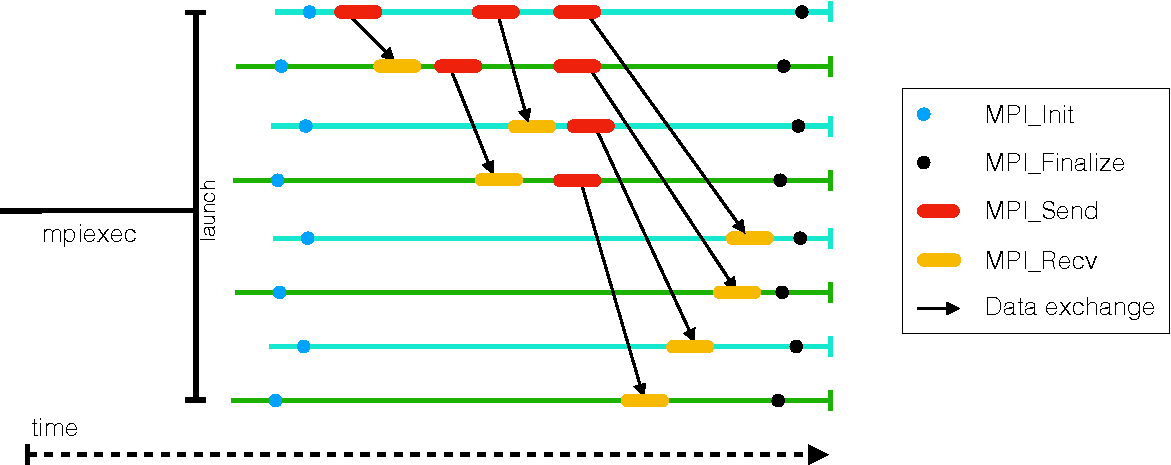
\includegraphics[width=0.95\textwidth]{figures/L19/CMDA3634FA19Broadcast-crop.pdf}
    \caption{Tree broadcast operation.}
    \label{broadcast.fig}
\end{figure}

The key to the broadcast tree is that as soon as a process has the message it keeps sending out the message to processes that have not received the message yet. We implement a tree base broadcast in the following code.

\begin{minted}{c}
void myBroadcast(int msgN, int *msgOut, int *msgIn, int msgTag){

  // find process rank and process count      
  int rank, size;
  MPI_Comm_rank(MPI_COMM_WORLD, &rank);
  MPI_Comm_size(MPI_COMM_WORLD, &size);

  int alive = 1;
  while(alive<size){ // loop over log2(size) rounds    
    int newAlive  = 2*alive;
    int msgDest   = rank + alive;
    int msgSource = rank - alive;

    if(rank<alive && msgDest<newAlive && msgDest<size){ // send   
      MPI_Send(msgOut, msgN, MPI_INT, msgDest, msgTag, MPI_COMM_WORLD);
    }

    if(rank<newAlive && msgSource>=0){
      MPI_Status msgStatus;
      MPI_Recv(msgIn, msgN, MPI_INT, msgSource, msgTag, MPI_COMM_WORLD, &msgStatus);
    }
    alive = newAlive;
  }
}
\end{minted}

Notice we first declare that there is just one ``alive'' process, our root process. Inside the \texttt{while} loop only the processes with rank smaller than \texttt{alive} send a message to processes with rank between \texttt{alive} and \texttt{2*alive}. In each round of the \texttt{while} loop the number of \texttt{alive} node doubles, and the number of messages also doubles. As soon as a process receives the message it is ``alive'' and keeps sending the message in all subsequent rounds of the \texttt{while} loop as long as its destination rank is valid.

Both the call tree based broadcast and the na\"{i}ve approach where the root process sequentially sends the message to all other processes require \texttt{P-1} messages. The difference is that in the tree based approach each rank only sends at most $\lceil\log_2(P)\rceil$ messages. Thus we say that the na\"{i}ve broadcast ``costs'' $\mathcal{O}(P)$ and the tree based broadcast costs $\mathcal{O}(\log_2(P))$. Here cost refers to the total number of rounds of communication. This makes sense for small messages since the constant of proportionality in the actual cost depends on the latency.

The manpage for the MPI implementation of the broadcast option, called \texttt{MPI\_Bcast}, is \href{https://www.mpich.org/static/docs/v3.1.x/www3/MPI_Bcast.html}{here}. In the following we nominate rank zero (relative to the communicator) to be the root process and send a single integer (likely through a call tree) to all other processes in the communicator. In this example we use \texttt{MPI\_COMM\_WORLD} for the communicator so all ranks will eventually receive the single integer message.

\begin{minted}{c}
 // see L19/mpiBroacast.c
 int msgN = 1;
 int *msgOut = (int*) malloc(msgN*sizeof(int));
 int msgRoot = 0;
 MPI_Bcast(msgOut, msgN, MPI_INT, msgRoot, MPI_COMM_WORLD);
\end{minted}

{\bf Note}: a common mistake when using collective operations like \texttt{MPI\_Bcast} is to not make sure that all processes call the function. If process that is supposed to receive and then send a message to another process that needs to receive the message then the function will deadlock.

\section{Reduction operation}

The second collective communication pattern we consider is the reduction: a value (or values) are accumulated from all ranks and the reduced result is deposited at the end on one process (which we will call the root process). We can think of this as applying a reduction operation to a distributed array of data. The reduction operation can be: compute the sum, product, minimum, maximum, logical or, logical and, logical exclusive or, of the entries in a distributed array. For example consider the case where all processes have a single value in their local array say set to their rank value. Then after a reduction on $P$ ranks:

\begin{align*}
    \mbox{reduction}_{\mbox{max}} &= P-1, \\
    \mbox{reduction}_{\mbox{min}} &= 0, \\
    \mbox{reduction}_{\mbox{sum}} &= P(P+1)/2, \\
    \mbox{reduction}_{\mbox{prod}} &= 0\times (P-1)!, \\
\end{align*}

A na\"{i}ve way to do this: all ranks send their message to the root process and that process applies the reduction operation to all the incoming value (or values) sequentially. If there are $P$ processes then it will take the root process $P$ message rounds to complete the broadcast and the root process will perform $\mathcal{O}(P)$ operations in the reduction. However, just like in the broadcast there is a missed opportunity here. This na\"{i}ve approach requires the root process to do all the arithmetic/logic operations in the logic while all the other ranks are just sending data. 

To reduce the cost of the parallel reduction we can reverse the phone tree approach we used in the broadcast tree algorithm. This time we nominate each of the top half of the processes to send their value to one of the bottom half of the processes. The receiving processes will apply the reduction operation (for instance sum) their own value and the value that they receive. We then halve the number of active processes through conditional statements and repeat the process. So we start with $P$ alive processes, then after the first round of communications only $P/2$ are alive, and after the second round only $P/4$ are alive. We repeat this process until there is just one process, namely the root process, that finalizes the calculation with incoming data and the computation is completed. 

At each stage of this algorithm the number of alive processes is halved thus it will take $\mathcal{O}(\log_2(P)$ rounds of messages to complete the tree based reduction and this improves on the $\mathcal{O}(P)$ cost of the na\"{i}ve algorithm. 


\myvbox[myexercise]{{\bf Exercise}: prove that the tree reduction only requires $P-1$ messages to be sent which is the same as the na\"{i}ve algorithm and thus does not increase the number of messages sent.}

\begin{figure}[htbp!]
    \centering
    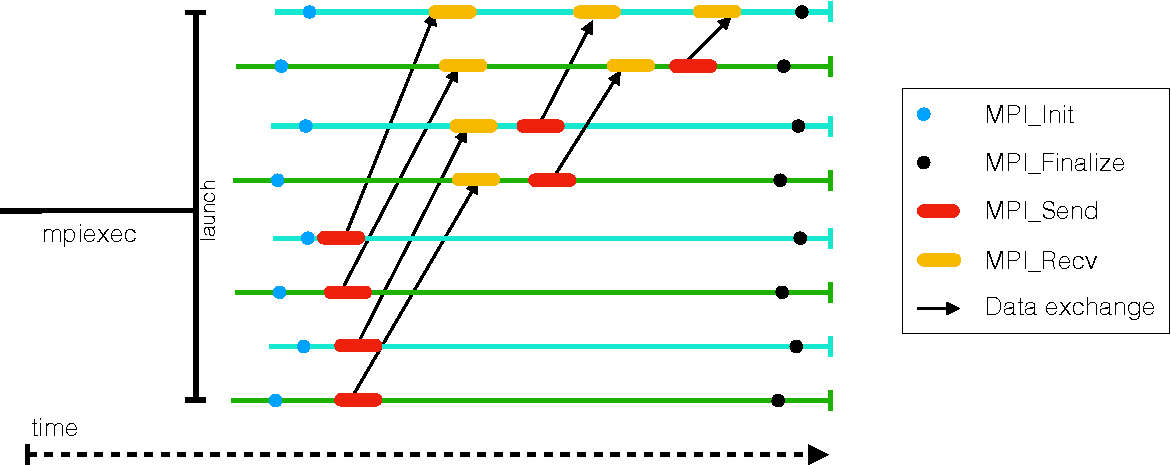
\includegraphics[width=0.95\textwidth]{figures/L19/CMDA3634FA19Reduction-crop.pdf}
    \caption{Tree reduction operation.}
    \label{reduction.fig}
\end{figure}

The tree reduction algorithm can be implemented using MPI send and receive function calls as follows

\begin{minted}{c}
// see L19/myReduce.c
void myReduce(int msgN, int *msgBuffer, int msgTag){

  // find process rank and process count                          
  int rank, size;
  MPI_Comm_rank(MPI_COMM_WORLD, &rank);
  MPI_Comm_size(MPI_COMM_WORLD, &size);

  int *msgTmp = (int*) calloc(msgN, sizeof(int));

  int alive = size;
  while(alive>1){
    int newAlive  = (alive+1)/2;
    int msgDest   = rank - newAlive;
    int msgSource = rank + newAlive;

    // recv from above              
    if(rank<newAlive && msgSource>=newAlive && msgSource<alive){ // send                                
      MPI_Status msgStatus;
      MPI_Recv(msgTmp, msgN, MPI_INT, msgSource, msgTag, MPI_COMM_WORLD, &msgStatus);

      // add incoming values to outgoing buffer                    
      for(int n=0;n<msgN;++n){
        msgBuffer[n] += msgTmp[n];
      }
    }

    // send down                           
    if(rank>=newAlive && rank<alive && msgDest<newAlive){
      MPI_Send(msgBuffer, msgN, MPI_INT, msgDest, msgTag, MPI_COMM_WORLD);
    }

    // update alive        
    alive = newAlive;
  }

  free(msgTmp);
}
\end{minted}
The reduction operations is another example of a very commonly used communication pattern and so the MPI standard provides an implementation callable through \texttt{MPI\_Reduce}.

\begin{minted}{c}
 // see L19/mpiReduce.c
 // prepare message                  
  int msgN = 1;
  int *msgBuffer  = (int*) malloc(msgN*sizeof(int));
  msgBuffer[0] = rank;

  // do sum reduction with MPI_Reduce  
  int *msgReduced = (int*) malloc(msgN*sizeof(int));
  int msgRoot = 0;
  MPI_Reduce(msgBuffer, msgReduced, msgN, MPI_INT, MPI_SUM, msgRoot, MPI_COMM_WORLD);
\end{minted}

{\bf Note}: if you want the result of the reduction operation to be distributed to all the ranks and not just the root process then you can use the \texttt{MPI\_Allreduce} variant.

\section{Barrier operation}

To round out the introduction to collective MPI primitives in this chapter we mention the barrier operation. The barrier operation requires all processes to have participated in the operation before any process exits the barrier operation. 

We can compose the reduction and broadcast operations in a moderately na\"{i}ve approach to form the barrier operation as shown in Figure \ref{barrier.fig}. First all processes participate in a tree based barrier. Once the root process completes we know that all processes have participated thus we follow the reduction operation by launching a broadcast from the root process. This basically amounts to the root process notifying all processes that all the processes had participated in the reduction stage. 
\begin{figure}[htbp!]
    \centering
    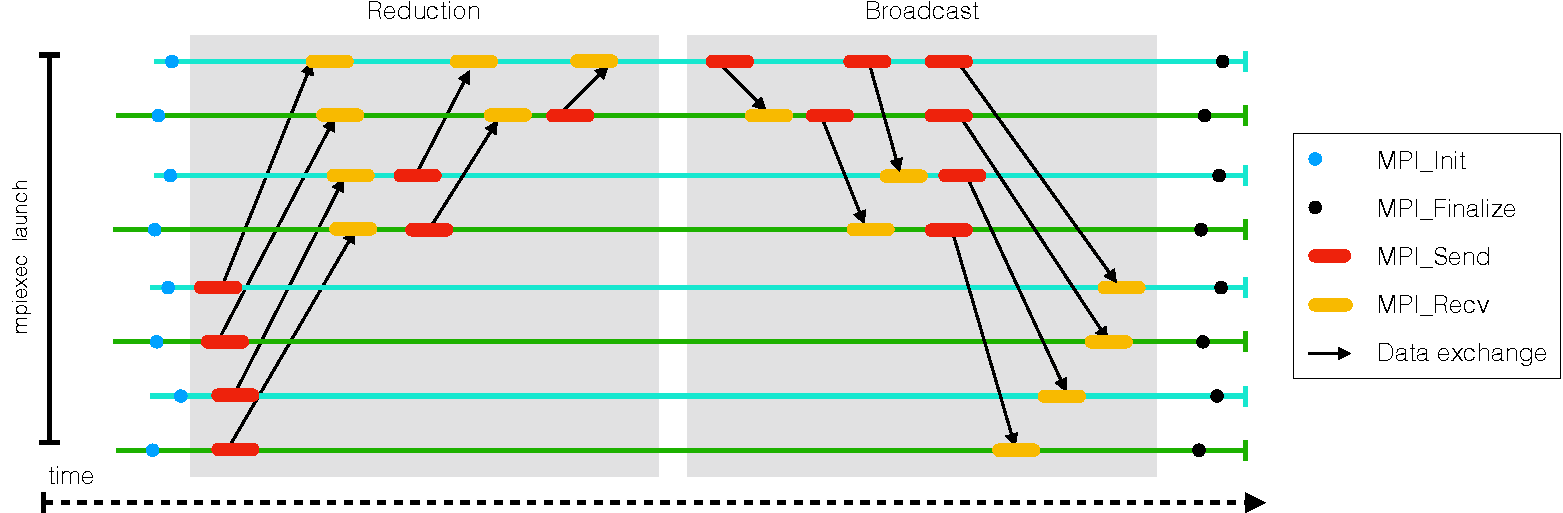
\includegraphics[width=0.95\textwidth]{figures/L19/CMDA3634FA19Barrier-crop.pdf}
    \caption{Tree barrier: we combine a reduction operation and a broadcast operation. After the broadcast every MPI process knows that all other ranks entered into the reduction. }
    \label{barrier.fig}
\end{figure}

As with the reduction and broadcast collective operations the barrier is a very useful operation. The \texttt{MPI\_Barrier} operation can be launched as follows.
\begin{minted}{c}
MPI_Barrier(MPI_COMM_WORLD);
\end{minted}

\section{Summary of MPI collective communications}

Table \ref{mpiCollectivesAPI.tab} summarizes useful MPI collective communication routines used above.

\begin{table}[htbp!]
    \centering
    \begin{tabular}{p{1.in}|p{5in}} \hline
      Action & Action implemented using MPI  functions\\ \hline
    Broadcast &  \texttt{MPI\_Bcast([BUFFER],[NUM DATA], [MPI DATA TYPE], [ROOT], [COMMUNICATOR]);} \\ \hline
    Reduction &\texttt{MPI\_Reduce([SEND BUFFER], [RECV BUFFER], [NUM DATA], [MPI DATA TYPE], [MPI OP], [ROOT], [COMMUNICATOR]);} \\ \hline
    All Reduction &\texttt{MPI\_Allreduce([SEND BUFFER], [RECV BUFFER], [NUM DATA], [MPI DATA TYPE], [MPI OP],  [COMMUNICATOR]);} \\ \hline
    Barrier & \texttt{MPI\_Barrier([COMMUNICATOR]);} \\
    \hline
    All to all & \texttt{MPI\_Alltoall([SEND BUFFER], [SEND COUNT], [MPI SEND TYPE], [RECV BUFFER], [RECV COUNT], [MPI RECV TYPE], [COMMUNICATOR]);} \\ \hline
    \end{tabular}
    \caption{Summary of commonly used MPI collective communication patterns. Here \texttt{[MPI COMMUNICATOR]} is an MPI Communicator struct, typically \texttt{MPI\_COMM\_WORLD}, i.e. the global communicator for all processes until we start using custom MPI Communicators. }    
    \label{mpiCollectivesAPI.tab}
\end{table}
